
\section{Dataset Overview}
To achieve high accuracy while minimizing computational time, we employed the \texttt{FASTPM} particle-mesh simulation code \citep{10.1093/mnras/stw2123} (See Section~\ref{sec:fastpm}).

In our study, we quantify super-sample covariance in higher-order statistics using two N-body simulations: \textbf{BIGBOX} and \textbf{TILED}. The \textbf{BIGBOX} simulation, conducted as part of the HalfDome project \citep{2024arXiv240717462B}, encompasses a large cosmic volume, whereas the \textbf{TILED} simulation represents a smaller volume with the same resolution as BIGBOX, specifically excluding large-scale modes. The cosmological parameters for both simulations align with those of IllustrisTNG \citep{2019ComAC...6....2N}, as listed in Table~\ref{tab:simulations}.

\begin{table}[h]
\centering
\begin{tabular}{lcc}
\toprule
\textbf{Parameter} & \textbf{Symbol} & \textbf{Value} \\
\midrule
Hubble constant & $H_0$ & 67.74 \, [$\mathrm{km\,s^{-1}\,Mpc^{-1}}$] \\ 
Matter density & $\Omega_m$ & 0.3089 \\
Baryon density & $\Omega_b$ & 0.0486 \\
Amplitude of fluctuations & $\sigma_8$ & 0.8159 \\
Spectral index & $n_s$ & 0.9667 \\
Sum of neutrino masses & $M_{\nu}$ & 0.0 \, [eV] \\
\bottomrule
\end{tabular}
\caption{Cosmological parameters used in the N-body simulations.}\label{tab:simulations}
\end{table}

The \textbf{BIGBOX} simulation models an extensive cubic volume of $L = 3750$ Mpc/h with $6144^3$ particles, enabling detailed capture of large-scale structures. From this data, a full-sky map was generated by first covering an octant of the sky and subsequently extending it to a full-sky projection.

The \textbf{TILED} simulation covers a smaller volume of $L = 625$ Mpc/h, populated with $1024^3$ particles. To achieve resolution parity with the BIGBOX simulation, volumes were replicated and tiled together, forming a full-sky map comparable in detail to the BIGBOX simulation but without the inclusion of large-scale modes.

Both simulations commence at an initial redshift of $z = 9$, utilizing an initial linear matter power spectrum at $z = 0$ generated via the \texttt{CLASS} code \citep{2011JCAP...07..034B}. This setup ensures consistency with observational data of the early universe. We evolved the simulations over 60 time steps, reaching the present day ($z = 0$), thereby capturing the non-linear growth of cosmic structures.

\begin{figure}[ht]
    \centering
    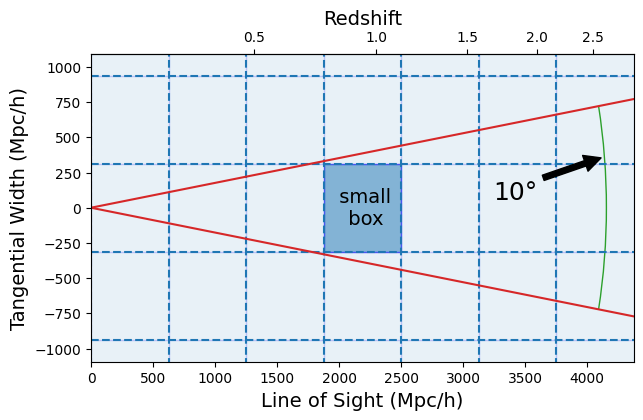
\includegraphics[width=0.6\textwidth]{figures/light_cone_configuration.png}
    \caption{Spatial and redshift setup for the \textbf{BIGBOX} and \textbf{TILED} simulations. The left side of the figure features red lines delineating the light cone boundaries, covering a $10^\circ$ field of view on the sky. Overlaid on this are dashed blue grids that partition the overall simulation volume into smaller, manageable tiling regions. Within these grids, the "small box" highlights a specific tiled region that resides inside the extensive BIGBOX volume. The horizontal axis represents the line-of-sight distance measured in comoving megaparsecs per $h$, with the corresponding redshift values displayed on the top axis.} \label{fig:simulationsetting}
\end{figure}
Figure~\ref{fig:simulationsetting} showcases the spatial and redshift setup for the \textbf{BIGBOX} and \textbf{TILED} simulations used in cosmological studies. 

\section{Generating Convergence Maps}
To simulate the weak lensing signals observed in surveys, we generated convergence maps from our N-body simulations. Light cones were constructed with particles inserted on-the-fly at the appropriate redshifts through interpolation between N-body time steps.

To balance computational efficiency with the need of accurancy, we set the width of each radial shell to $\Delta a = 0.01$, corresponding to a comoving distance of approximately $\Delta \chi \approx 100 \, h^{-1} \, \text{Mpc}$.

For each shell, the three-dimensional matter density $\delta(\mathbf{x}, z_i)$ was projected onto a two-dimensional plane perpendicular to the line of sight. The projected surface density $\Sigma(\hat{\mathbf{n}}, \chi_i)$ at an angular position $\hat{\mathbf{n}}$ was computed by integrating the matter density within the shell along the radial direction:
\begin{equation}
    \Sigma(\hat{\mathbf{n}}, \chi_i) = \int_{\chi_i}^{\chi_{i+1}} \delta(\chi \hat{\mathbf{n}}, z(\chi)) \, d\chi.
\end{equation}
In practice, the surface density was mapped onto a HEALPix grid \citep{Górski_2005} to create a full-sky map $\Sigma(n_j, \chi_i)$, where $n_j$ represents discretized angular positions. The HEALPix grid resolution was set to $N_{\text{side}} = 8192$, providing an angular resolution of approximately $0.43$ arcminutes, which is sufficient to capture small-scale structures relevant to weak lensing studies.

The convergence $\kappa(n_j; z_s)$ at each pixel of the HEALPix grid was then obtained by summing contributions from all the shells up to the source redshift:
\begin{equation}
    \kappa(n_j; z_s) = \sum_{i} W(\chi_i, \chi_s) \Sigma(n_j, \chi_i) \Delta \chi_i,
\end{equation}
where $W(\chi, \chi_s)$ is the lensing efficiency function.
The effective comoving distance to the center of the $j$-th shell, $\chi^j$, is calculated as \citep{2015MNRAS.453.3043S}:
\begin{equation}
    \chi^j = \frac{\int_{\chi_{\min}}^{\chi_{\max}} \chi^3 \, \mathrm{d}\chi}{\int_{\chi_{\min}}^{\chi_{\max}} \chi^2 \, \mathrm{d}\chi} = \frac{3}{4} \frac{\chi_{\max}^4 - \chi_{\min}^4}{\chi_{\max}^3 - \chi_{\min}^3},
\end{equation}
The density contrast within the $i$-th pixel of the $j$-th shell, $\delta^j(\hat{\boldsymbol{n}}_i)$, is determined by:
\begin{equation}
    \delta^j(\hat{\boldsymbol{n}}_i) = \frac{n_{\mathrm{part}, i}^j}{\bar{n}_{\mathrm{part}}^j} - 1,
\end{equation}
where $n_{\mathrm{part}, i}^j$ is the number of particles in the $i$-th pixel of the $j$-th shell, and $\bar{n}_{\mathrm{part}}^j$ is the average number of particles per pixel in that shell.

We considered source redshifts $z_s$ from 0.5 to 2.5 in increments of 0.5, covering the range of distances relevant for current and future galaxy surveys, such as DES, LSST, \textit{Euclid}, and \textit{Roman}.

\begin{figure}
    \centering
    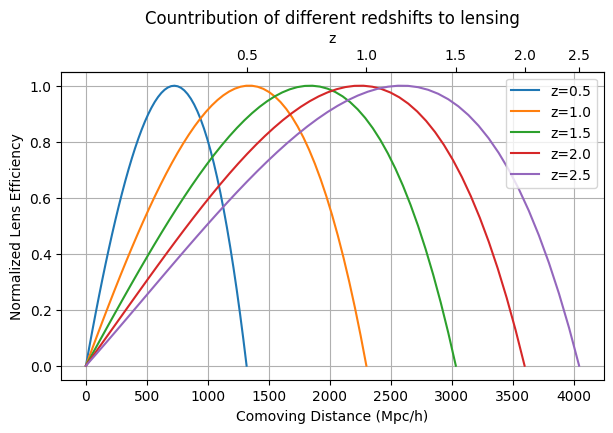
\includegraphics[width=0.6\textwidth]{figures/lensefficiency.png}
    \caption{Normalized lensing efficiency as a function of comoving distance for multiple source redshifts. The lensing efficiency peaks at intermediate comoving distances, indicating regions where the distribution of matter enhances the gravitational lensing signal.} \label{fig:lensing_efficiency}
\end{figure}
Figure~\ref{fig:lensing_efficiency} presents the normalized lensing efficiency as a function of comoving distance (measured in Mpc/$h$) for multiple source redshifts ($z$). The lensing efficiency curves exhibit peaks at intermediate comoving distances, indicating the regions where the distribution of matter along the line of sight most significantly enhances the gravitational lensing signal. 

\section{Incorporating Noise}
In real observations, measurements of the lensing signal are contaminated by noise arising from the intrinsic shapes of galaxies and errors in shape measurements. This noise, referred to as shape noise, constitutes a significant source of uncertainty, particularly on small angular scales.

We considered four different surveys with varying galaxy number densities, as detailed in Table~\ref{tab:survey_comparison}.
The variance of the shape noise per pixel was calculated as:
\begin{equation}
    \sigma_{\kappa, \text{noise}}^2 = \frac{\sigma_{\epsilon}^2}{2 n_{\mathrm{gal}} A_{\mathrm{pix}}},
\end{equation}
where $\sigma_{\epsilon}$ is the intrinsic ellipticity dispersion of galaxies, set to $\sigma_{\epsilon} = 0.26$ \citep{2019A&A...627A..59E}, $n_{\mathrm{gal}}$ is the galaxy number density per square arcminute, and $A_{\mathrm{pix}}$ is the solid angle of a pixel, set to $0.43$ arcminutes$^2$.
We generated a Gaussian random field $n(\hat{\mathbf{n}})$ with the calculated variance and added it to the convergence maps:
\begin{equation}
    \kappa_{\mathrm{obs}}(\hat{\mathbf{n}}) = \kappa(\hat{\mathbf{n}}) + n(\hat{\mathbf{n}}).
\end{equation}

\section{Patch Extraction for Analysis}
In order to simlplify the analysis onto a flat patch, we extracted patches from the full-sky convergence maps. Each patch covers an area of $10^\circ \times 10^\circ$ and is uniformly distributed across the sky using a Fibonacci grid \citep{2006QJRMS.132.1769S, 2023MNRAS.524.5591F}. The center of each patch is positioned at the vertices of the Fibonacci grid defined by golden ratio spirals:
\begin{equation}
    \sin \theta_i = \frac{2i}{2N + 1}, \quad \phi_i = \frac{2 \pi i}{\varphi}, \quad -N \leq i \leq N, \quad -\frac{\pi}{2} \leq \theta_i \leq \frac{\pi}{2},
\end{equation}
where $N$ is the number of patches and $\varphi = (1 + \sqrt{5})/2$ is the golden ratio.

The number of patches, denoted \( N_{\text{patches}} \), was optimized to ensure that individual patches do not overlap, except in regions near the poles where overlapping patches were subsequently discarded. The optimization process commenced with an initial count of \( N_{\text{patches}} = 400 \) and involved iteratively reducing this number until a configuration was achieved wherein the patches remained non-overlapping, except for centers located within \( 10\sqrt{2}^\circ \, \mathrm{\deg}\) of the poles, that is $|\theta_i| \geq 10\sqrt{2}^\circ$ and $|\phi_i| \leq \pi - 10\sqrt{2}^\circ$. Additionally, patches include points heavily tiled along with line of sight and near the equator are excluded to avoid severe Box Replication Effect (see Sec.~\ref{sec:boxreplication} for further check).
After optimization and masking, the number of patches was set to $N_{\text{patches}} = 273$, effectively reducing to $N_{\text{patches}} = 262$, effectively cover $64 \%$ of the sky. The visualization of the Fibonacci grid is shown in Figure~\ref{fig:fibonacci}.
\begin{figure}[ht]
    \centering
    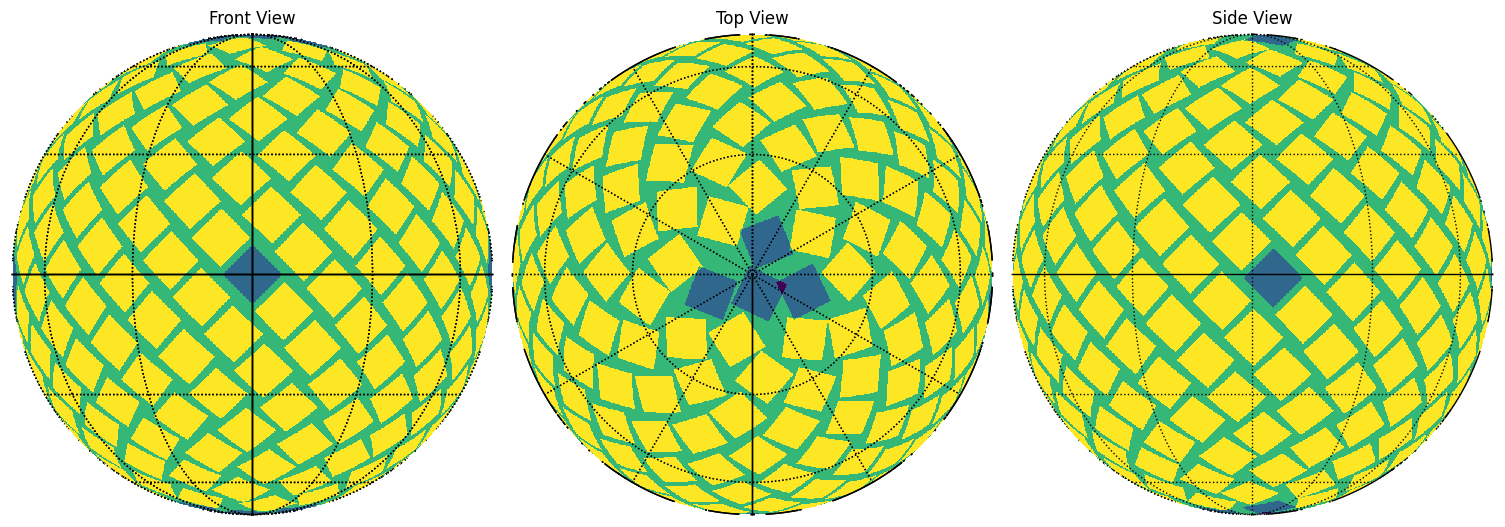
\includegraphics[width=0.8\textwidth]{figures/fibonacci_grid.png}
    \caption{Visualization of the Fibonacci grid with $N_{\text{patches}} = 273$ patches, each covering approximately $10 \times 10$\,deg$^2$. 
    After the optimization and masking, the number of patches is reduced to $N_{\text{patches}} = 262$, effectively covering $64 \%$ of the sky.
    Each panel show the patches distribution on the Front, Top and Side view.}\label{fig:fibonacci}
\end{figure}

To verify the absence of overlap between patches, we calculated the vertices of each patch and conducted pairwise overlap checks with all other patches. For a Fibonacci grid center characterized by coordinates \( (\theta_i, \phi_i) \), the vertices of the corresponding patch are defined as:
\begin{align}
    \left( \theta_i - \Delta \theta,\, \phi_i - \Delta \phi \right), \quad &\left( \theta_i - \Delta \theta,\, \phi_i + \Delta \phi \right), \nonumber \\
    \left( \theta_i + \Delta \theta,\, \phi_i - \Delta \phi \right), \quad &\left( \theta_i + \Delta \theta,\, \phi_i + \Delta \phi \right),
\end{align}
where
\begin{align}
    \Delta \theta = 5\sqrt{2}\, \mathrm{\deg}, \quad \Delta \phi = 5\sqrt{2}\sin \theta_i \, \mathrm{\deg}.
\end{align}

Using the vertices of the Fibonacci grid as centers, we employed the \texttt{gnomview} function from the \texttt{healpy} library \citep{Zonca2019} to project each spherical patch onto a flat plane via a gnomonic projection. Each patch is represented by a $2048 \times 2048$ grid of pixels, resulting in a pixel size of:
\begin{equation}
    \Delta \theta = \frac{10^\circ}{2048} \approx 0.00488^\circ \approx 0.293' \quad \text{per pixel}.
\end{equation}

The analysis utilizes 11 realizations from the BIGBOX simulation and 20 realizations from the TILED simulation. For each realization, the covariance is computed using 262 patches extracted from the full-sky map of each simulation.
Therefore, we obtain a total of 2882 patches from the BIGBOX simulation and 5240 patches from the TILED simulation. 

\section{Gaussian Smoothing}
Shape noise predominantly affects small angular scales. To mitigate this noise and enhance the detection of the underlying lensing signal, we applied Gaussian smoothing to the noisy convergence maps. The Gaussian filter used is defined by:
\begin{equation}
    W(\theta) = \frac{1}{\pi \theta_{\mathrm{G}}^2} \exp\left( -\frac{\theta^2}{\theta_{\mathrm{G}}^2} \right),
\end{equation}
where $\theta$ is the angular distance from the center of the filter, and $\theta_{\mathrm{G}}$ is the smoothing scale. For our analysis, we selected $\theta_{\mathrm{G}} = 2'$, $5'$, $8'$, and $10'$.

By convolving the noisy convergence map with the Gaussian filter, we obtained the smoothed convergence map:
\begin{equation}
    \kappa_{\mathrm{smoothed}}(\hat{\mathbf{n}}) = \int d\Omega' \, W(|\hat{\mathbf{n}} - \hat{\mathbf{n}}'|) \kappa_{\mathrm{obs}}(\hat{\mathbf{n}}').
\end{equation}

Figure~\ref{fig:smoothing} demonstrates the application of Gaussian smoothing to a noisy convergence map. The figure presents four panels, each corresponding to a different smoothing scale: $\theta_{\mathrm{G}} = 2'$, $5'$, $8'$, and $10'$. As the smoothing scale increases, the convolution with the Gaussian filter effectively reduces small-scale noise, as evidenced by the diminishing small-scale fluctuations in the map. 
\begin{figure}[ht]
    \centering
    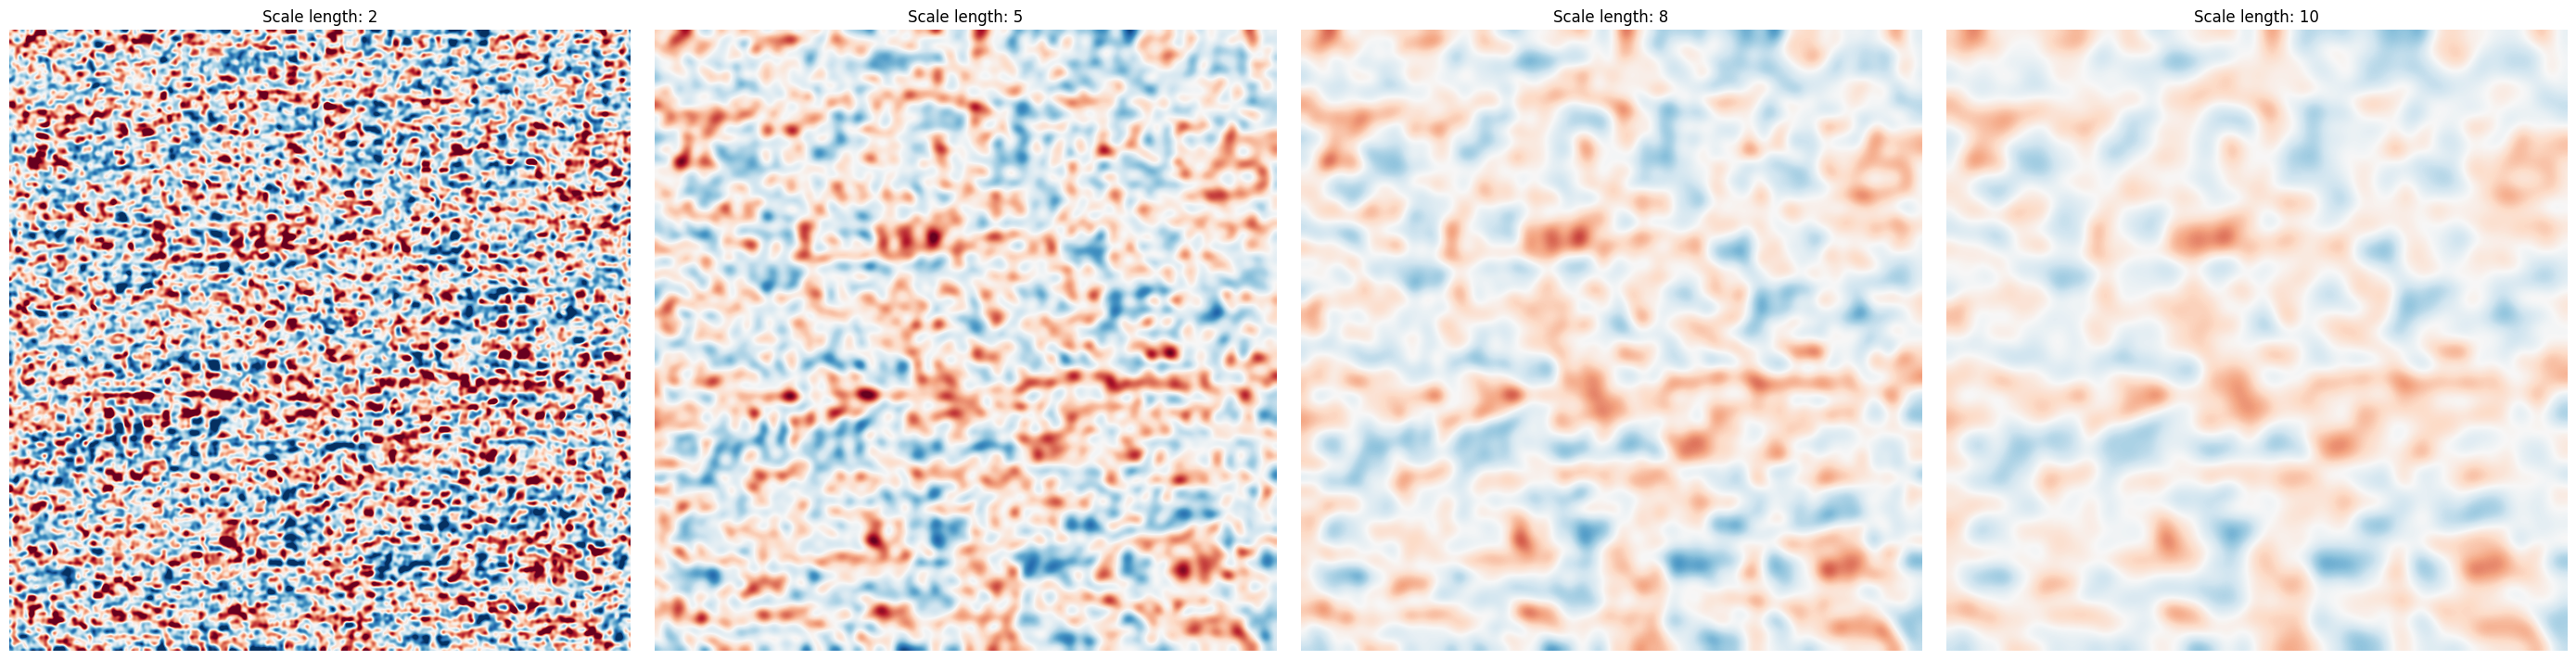
\includegraphics[width=\textwidth]{figures/smoothed_comparison.png}
    \caption{Effect of Gaussian smoothing on a noisy convergence map. Each panel shows the result of applying a Gaussian filter with a different smoothing scale $\theta_{\mathrm{G}} = 2'$, $5'$, $8'$, and $10'$. As the smoothing scale increases, small-scale noise is progressively suppressed, and large-scale structures become more prominent. This demonstrates how Gaussian smoothing effectively reduces shape noise while enhancing the detection of the underlying lensing signal.}
\label{fig:smoothing}
\end{figure}

\section{Measurements}
In order to characterize the influence of super-sample covariance on higher-order statistics, this study concentrates on the bispectrum, probability distribution function (PDF), peak counts, minima counts, and Minkowski functionals. These statistical measures offer complementary insights into the underlying matter distribution and exhibit sensitivity to distinct features of the gravitational lensing signal.

\subsection{Statistical Measures and Computational Methods}
Table~\ref{tab:statistics} delineates the range of values and the computational subroutines employed for each statistical measure. Each statistic is computed both for full-sky analyses and sky patches, utilizing the appropriate methodologies as specified.
\begin{table*}[htbp]
    \centering
    \begin{tabular}{lcc}
    \toprule
    \textbf{Statistic} & \textbf{Range} & \textbf{Subroutine (Sky Patch)} \\
    \midrule
    Angular Power Spectrum & $300 \leq \ell \leq 3000$ & \texttt{lenstools.powerSpectrum} \\
    Bispectrum & $300 \leq \ell \leq 3000$ & \texttt{lenstools.bispectrum} \\
    Peak Counts & $-4 \leq \kappa/\sigma_\kappa \leq 4$ & \texttt{lenstools.peakCount} \\
    Minima Counts & $-4 \leq \kappa/\sigma_\kappa \leq 4$ & \texttt{lenstools.peakCount} \\
    Probability Distribution Function (PDF) & $-4 \leq \kappa/\sigma_\kappa \leq 4$ & \texttt{lenstools.pdf} \\
    Minkowski Functionals & $-4 \leq \kappa/\sigma_\kappa \leq 4$ & \texttt{lenstools.minkowskiFunctionals} \\
    \bottomrule
    \end{tabular}
    \caption{Summary of the statistical measures employed in this investigation, including their respective value ranges and computational subroutines utilized for both full-sky and sky-patch analyses.}\label{tab:statistics}
\end{table*}
The angular power spectrum, denoted as $C_{\ell}^{\kappa\kappa}$, alongside three configurations of the bispectrum, $B_{\ell_1\ell_2\ell_3}^{\kappa\kappa\kappa}$, are derived from unsmoothed convergence maps. The bispectrum calculations encompass three distinct configurations: equilateral ($\ell_1 = \ell_2 = \ell_3$), squeezed ($\ell_1 = \ell_2 = 10\ell_3$), and isosceles ($\ell_1 = \ell_2 = 2\ell_3$). 
All bispectrum and angular power spectrum computations are confined within the multipole range $\ell \in [300, 3000]$ with eight bins, consistent with the multipole selection in the HSC Y3 cosmic shear analysis \citep{2023PhRvD.108l3519D}. We adopt a logarithmic binning approach to effectively sample the range of scales, dividing the multipole interval into 8 bins that are evenly spaced in logarithmic space. 

Conversely, the PDF, peak counts, minima counts, and Minkowski functionals are derived from smoothed convergence maps, where the smoothing angle is fixed at 2 arcminutes for the primary results. These measurements are conducted within the normalized range $-4 \leq \kappa/\sigma_{\kappa} \leq 4$, linearly divided into 8 bins following \citet{2021A&A...648A.115M}. $\sigma_{\kappa}$ denotes the standard deviation of each patch's convergence map.

All statistical computations are performed using the \texttt{lenstools} package \citep{2016A&C....17...73P}.

\subsection{Covariance Matrix Estimation}
Following the measurement phase, this study examines the influence of super-sample covariance on the covariance matrices associated with the aforementioned statistical measures. To achieve this, we employ an unbiased estimator for the covariance matrix as previously defined in Equation~\ref{eq:covariance}. 

Additionally, we also compute the correlation matrix for each statistical measure to investigate the interdependence between different scales and configurations. The correlation matrix is defined as:
\begin{equation}
    \rho_{ij} = \frac{\text{Cov}(\mathcal{O}_i, \mathcal{O}_j)}{\sqrt{\text{Cov}(\mathcal{O}_i, \mathcal{O}_i)\text{Cov}(\mathcal{O}_j, \mathcal{O}_j)}},
\end{equation}
where $\mathcal{O}_i$ and $\mathcal{O}_j$ represent the $i$-th and $j$-th statistical measures, respectively.

After the covariance and correlation matrices are computed for both the BIGBOX and TILED simulations, we compare the matrices to quantify the impact of super-sample covariance on the statistical measures. The comparison is conducted by calculating the ratio between the covariance and correlation matrices of the BIGBOX and TILED simulations. 

In the case of correlation matrices, we exclude the diagonal elements---since they are always unity---when calculating the ratio. For covariance matrices, the ratio is calculated over the entire matrix. 

Regarding $\ell$-binned statistics, we determine the ratio across all bins. For $\nu$-binned statistics, we exclude the first and last bins from the ratio calculation due to their limited data points and unreliability.